\documentclass[border=10pt]{standalone}
\usepackage{amsmath}
\usepackage{tikz}
\usetikzlibrary{arrows.meta, decorations.pathmorphing}

\begin{document}
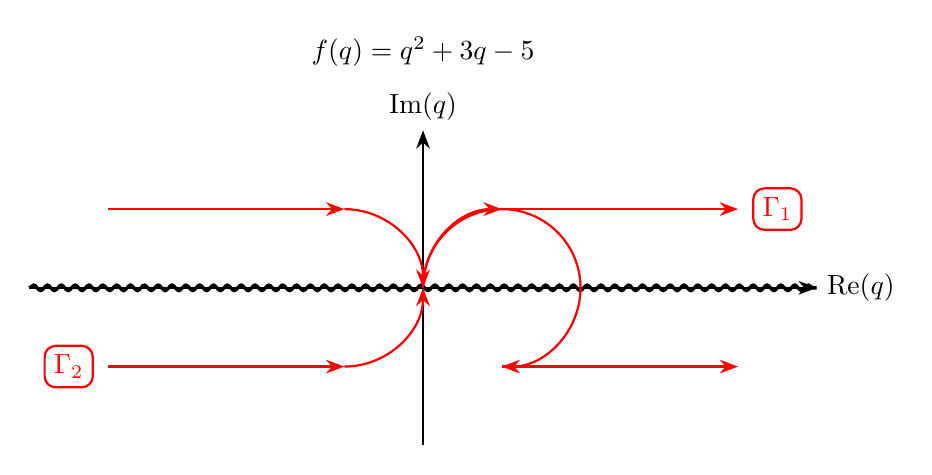
\begin{tikzpicture}[>=Stealth, thick]
    % Axes
    \draw[->] (-5,0) -- (5,0) node[right] {$\text{Re}(q)$};
    \draw[->] (0,-2) -- (0,2) node[above] {$\text{Im}(q)$};
    
    % Function
    \node at (0,3) {$f(q) = q^2 + 3q - 5$};
    
    % Branch Cut
    \draw[decorate, decoration={snake, segment length=5pt, amplitude=1pt}, very thick] (-5,0) -- (5,0);
    
    % Path Gamma1
    \draw[red, ->] (-4,1) -- (-1,1);
    \draw[red, ->] (-1,1) arc (90:0:1);
    \draw[red, ->] (0,0) arc (180:90:1);
    \draw[red, ->] (1,1) -- (4,1);
    \node[red, draw, rounded corners, fill=white] at (4.5,1) {$\Gamma_1$};
    
    % Path Gamma2
    \draw[red, ->] (-4,-1) -- (-1,-1);
    \draw[red, ->] (-1,-1) arc (-90:0:1);
    \draw[red, ->] (0,0) arc (180:-90:1);
    \draw[red, ->] (1,-1) -- (4,-1);
    \node[red, draw, rounded corners, fill=white] at (-4.5,-1) {$\Gamma_2$};
\end{tikzpicture}
\end{document}